% !TEX root = ./Vorlesungsmitschrift AGLA 2.tex  
\lecture{Fr 08.05. 10:15}{}
\begin{definition*}
    Sei \( K \) ein Körper. Wir nennen eine Bijektion \( \alpha\maps K\to K \) einen Automorphismus von \( K \) falls gilt
    \begin{align*}
        \alpha(\lambda+\mu)&=\alpha(\lambda)+\alpha(\mu)\quad \forall \lambda,\mu\in K
        \intertext{und}
        \alpha(\lambda\cdot \mu)&=\alpha(\lambda)\cdot \alpha(\mu)\quad \forall  \lambda,\mu\in K
    \end{align*}
\end{definition*}
\begin{beispiel}
    \begin{align*}
        K=\rationals(\sqrt{2})=\Set{x+y\sqrt{2}|x,y\in\rationals}
    \end{align*}
    ist ein Körper und 
    \begin{align*}
        \alpha\maps \begin{aligned}[t]
            \rationals(\sqrt{2})&\to \rationals(\sqrt{2})\\
            x+y\sqrt{2}&\mapsto x-y\sqrt{2}.
        \end{aligned}
    \end{align*}
\end{beispiel}
\begin{satz}\label{alle_automorphismen_auf_r_identitaet}
    Sei \( \alpha\maps \reals\to \reals \) ein Automorphismus von \( \reals \). Dann gilt \( \alpha=\Id_{\reals} \).
\end{satz}
\begin{proof}
    Sei \( \alpha\maps \reals\to \reals \) ein Automorphismus.
    \begin{proofenumerate}
        \item Dann gilt
        \begin{align*}
            \alpha(0)=\alpha(0+0)=\alpha(0)+\alpha(0),
        \end{align*}
        also \( \alpha(0)=0 \).
        \item Dann gilt
        \begin{align*}
            0=\alpha(0)=\alpha(\lambda-\lambda)=\alpha(\lambda)+\alpha(-\lambda),
        \end{align*}
        also \( \alpha(-\lambda)=-\alpha(\lambda)\logicspace \forall \lambda\in \reals \).
        \item Dann gilt
        \begin{align*}
            \alpha(1)=\alpha(1\cdot 1)=\alpha(1)\alpha(1),
        \end{align*}
        also \( \alpha(1)=1 \) und daher
        \begin{align*}
            \alpha(n)=n\logicspace \forall n\in \wholes,
        \end{align*}
        \zb
        \begin{align*}
            \alpha(2)=\alpha(1+1)=\alpha(1)+\alpha(1)=1+1=2.
        \end{align*}
        \item Sei \( p\in \wholes \), \( q\in \naturals \), dann gilt
        \begin{align*}
            q\alpha\left( \frac{p}{q} \right)\begin{aligned}[t]
                &=\alpha(q)\alpha\left( \frac{p}{q} \right)=\alpha\left( q\frac{p}{q} \right)=\alpha(p)=p,
            \end{aligned}
        \end{align*}
        also \( \alpha\left( \frac{p}{q}=\frac{p}{q} \right) \) oder \( \alpha(t)=t\quad \forall t\in \rationals \).
        \item Sei \( \lambda\in \reals_{>0} \). Dann \texists  \( \mu\in\reals \) mit \( \lambda=\mu^2 \) und
        \begin{align*}
            \alpha(\lambda)=\alpha(\mu^2)=\alpha(\mu)\cdot \alpha(\mu)>0,
        \end{align*}
        also
        \begin{align*}
            \alpha(\lambda)>0\quad \forall \lambda\subset \reals>0.
        \end{align*}
    \end{proofenumerate}
    Wir zeigen nun \( \alpha(\lambda)=\lambda\quad \forall \lambda\in \reals \).

    \minisec{Gegenannahme}
    Sei \( \lambda\in \reals \) mit \( \alpha(\lambda)\neq \lambda \). Wir diskutieren den Fall \( \alpha(\lambda)<\lambda \) (\( \alpha(\lambda)>\lambda \) geht genauso).

    Wähle \( \frac{p}{q}\in \rationals \) mit
    \begin{align*}
        \alpha(\lambda)<\frac{p}{q}<\lambda.
    \end{align*}
    Dann gilt
    \begin{align*}
        \alpha(\lambda-\frac{p}{q})=\alpha(\lambda)-\frac{p}{q}<0
    \end{align*}
    \contra zu \( \lambda-\frac{p}{q}>0 \).
\end{proof}

\subsection*{Eine Familie von Kollineationen}
\begin{idee*}
    Wir verallgemeinern \thref{kollinieationen:beispiele:komplexe_konjugation}, um eine größere Klasse an Kollineationen zu erhalten als Affinitäten.
\end{idee*}
\begin{beispiel}
    \begin{align*}
        f\maps \begin{aligned}[t]
            \complexs^2&\to \complexs^2\\
            (x,y)&\mapsto (\conj{x},\conj{y})
        \end{aligned}
    \end{align*}
    respektiert Addition, \dh
    \begin{align*}
        f(z+z')=f(z)+f(z')\quad \forall z,z'\in \complexs^2,
    \end{align*}
    und hat die Eigenschaft
    \begin{align*}
        f(\lambda z)=\conj{\lambda} f(z)\quad \forall \lambda\in \complexs\logicspace \forall z\in \complexs^2.
    \end{align*}
    \tto Wir nennen \( f \) semilinear.
\end{beispiel}
\begin{definition*}
    Seien \( V,W \) Vektorräume über einem Körper \( K \). Wir nennen eine Abbildung \( F\maps V\to W \) \emph{semilinear}, wenn es einen Automorphismus \( \alpha \) von \( K \) gibt, sodass gilt
    \begin{itemize}
        \item \(F(v+v')=F(v)+F(v')\quad \forall v,v'\in V\)
        \item \( F(\lambda v)=\alpha(\lambda) F(v)\quad \forall \lambda\in K \logicspace \forall v\in V\).
    \end{itemize}
\end{definition*}
\begin{definition*}
    Seien \( X,Y \) affine Räume über einem Körper \( K \). Wir nennen eine Abbildung
    \begin{align*}
        f\maps X\to Y
    \end{align*}
    \emph{semiaffin}, wenn es eine \emph{semilineare Abbildung} \( F\maps T(X)\to T(Y) \) gibt mit
    \begin{align*}
        \vv{f(p) f(q)}=F(\vv{pq})\logicspace \forall p,q\in X.
    \end{align*}
    Falls \( f \) außerdem bijektiv ist, dann nennen wir \( f \) eine Semiaffinität.
\end{definition*}
\file{Hauptsatz affine Geometrie}
\begin{lemma}
    Sei \( f\maps X\to X \) eine Semiaffinität eines affinen Raumes \( X \). Dann ist \( f \) eine Kollineation.
\end{lemma}
\begin{proof}[Beweisidee]
    Sei \( \ell \subseteq X \) eine Gerade, \( p_0\in \ell \). Dann ist
    \begin{align*}
        T(\ell)=\Set{\vv{p_0 x}, x\in \ell}\subseteq T(x)
    \end{align*}
    ein \( K \)-Untervektorraum mit
    \begin{align*}
        \dim-{K}{T(\ell)}=1.
    \end{align*}
    Sei \( F\maps T(X)\to T(X)  \) die zu \( f \) gehörige semilineare Abbildung.

    Wir betrachten 
    \begin{align*}
        T(f(\ell))
        \begin{aligned}[t]
            &=\Set{\vv{f(p_0) f(x), x\in \ell}}\\
            &=\Set{F(\vv{p_0 x}), x\in \ell}
            &=F(T(\ell)).
        \end{aligned}        
    \end{align*}
    Dann ist auch \( F(T(\ell))\subseteq T(X) \) ein \( \explain{\text{Übung}}{K \text{-Untervektorraum}} \) der Dimension \( 1 \), also
    \begin{align*}
        f(\ell)\subseteq X
    \end{align*}
    eine Gerade.
\end{proof}
\begin{frage*}
    Gibt es Kollineationen, die keine Semiaffinität sind?
\end{frage*}
\tto Ja, \zb für \( \affindim-{X}=1 \).
\subsection*{Hauptsatz der affinen Geometrie}

Sei \( K \) ein Körper mit \( \anzahl-{K}\geq 3 \), \( X \) ein affiner Raum über \( K \) mit \( \affindim{X}\geq 2 \) und \( f\maps X\to X \) eine Kollineation. Dann ist \( f \) eine Semiaffinität.

\begin{bemerkung*}
    Aus \thref{alle_automorphismen_auf_r_identitaet} folgt, dass über \( \reals \) jede semilineare Abbildung linear ist.
\end{bemerkung*}
\begin{korollar*}
    Sei \( X \) ein affiner Raum über \( \reals \) mit \( \affindim{X}\geq 2 \), \( f\maps X\to X \) eine Kollineation. Dann ist \( f \) eine Affinität.
\end{korollar*}
\file{Quadriken erster Teil}
\section{Quadriken}
\begin{motivation*}
    Affine Unterräume der \( \reals^n \) sind gegeben durch \emph{lineare} Gleichungssysteme.
\end{motivation*}
\minisec{Jetzt:}
Betrachte den Unterraum im \( \reals^n \), der entsteht als Lösungsmenge einer \emph{quadratischen} Gleichung.
\begin{beispiele*}[im \( \reals^2 \)]
    \begin{enumerate}
        \item der Kreis
        \begin{align*}
            \Set{(x,y)\in \reals^2|x^2+y^2=1}
        \end{align*}
        \item Ellipsen, \( a,b>0 \)
        \begin{align*}
            E=\Set{(x,y)\in \reals^2|ax^2+by^2=1}
        \end{align*}
        \begin{figure}[H]
            \centering
            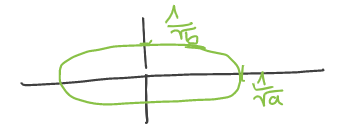
\includegraphics[width=0.5\linewidth]{figures/quadriken_beispiel_ellipse}
            \label{fig:quadriken_beispiel_ellipse}
        \end{figure}
        \item Parabel
        \begin{align*}
            y=ax^2
        \end{align*}
        \begin{figure}[H]
            \centering
            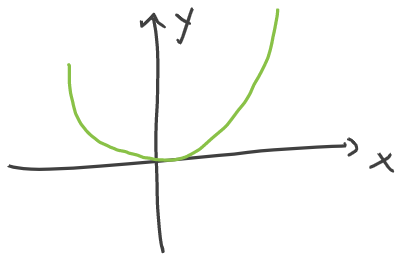
\includegraphics[width=0.5\linewidth]{figures/quadriken_beispiel_parabel}
            \label{fig:quadriken_beispiel_parabel}
        \end{figure}
        \item Hyperbeln, \( a,b>0 \)
        \begin{align*}
            ax^2-by^2=1 
        \end{align*}
        \begin{figure}[H]
            \centering
            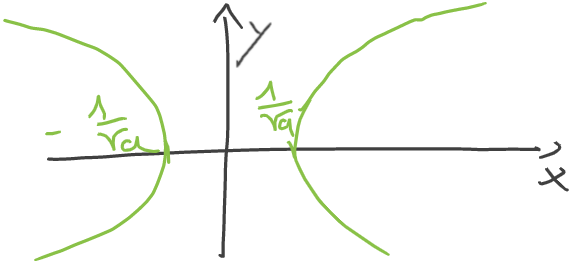
\includegraphics[width=0.5\linewidth]{figures/quadriken_beispiel_hyperbeln}
            \label{fig:quadriken_beispiel_hyperbeln}
        \end{figure}
        \item \( x^2=0 \)
        \begin{figure}[H]
            \centering
            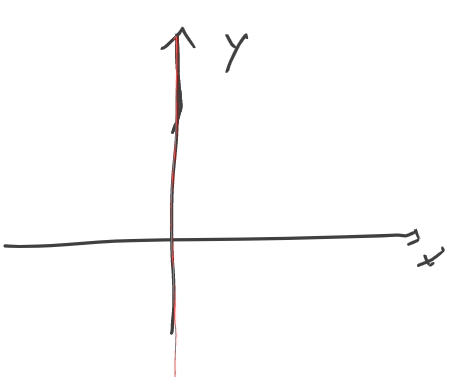
\includegraphics[width=0.4\linewidth]{figures/quadriken_beispiel_y_achse}
            \label{fig:quadriken_beispiel_y_achse}
        \end{figure}
        \item \( xy=0 \)
        \begin{figure}[H]
            \centering
            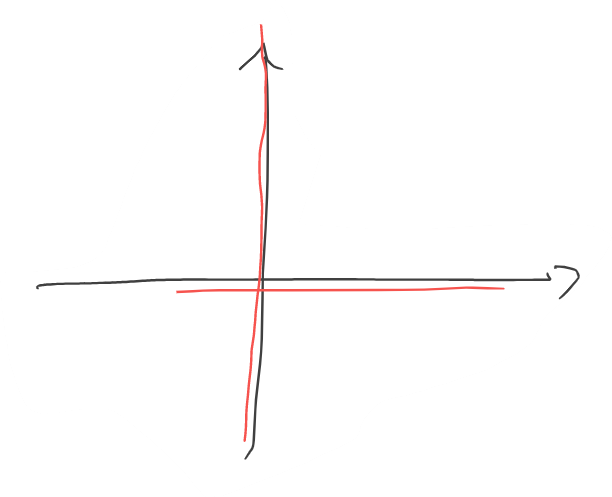
\includegraphics[width=0.4\linewidth]{figures/quadriken_beispiel_x_achse_und_y_achse}
            \label{fig:quadriken_beispiel_x_achse_und_y_achse}
        \end{figure}
        \item \( x^2+y^2=0 \)
        \begin{figure}[H]
            \centering
            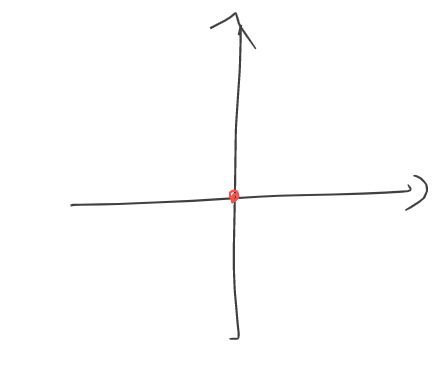
\includegraphics[width=0.4\linewidth]{figures/quadriken_beispiel_ursprung}
            \caption*{Der Ursprung}
            \label{fig:quadriken_beispiel_ursprung}
        \end{figure}
    \end{enumerate}
\end{beispiele*}
\begin{beispiele*}
    Sei \( Q\subseteq \reals^2 \) gegeben durch
    \begin{align*}
        x_1^2+2x_1x_2+2x_2^2+2x_1=0.
    \end{align*}
    Erster Schritt: Entferne den \enquote{gemischten} Term \( x_1 x_2 \).
    \begin{align*}
        (x_1+x_2)^2+x_2^2+2x_1=0.
    \end{align*}
    Nach der Koordinatentransformation
    \begin{align*}
        y_1=x_1+x_2\quad y_2=x_2
    \end{align*}
    ist \( Q \) gegeben durch
    \begin{align*}
        y_1^2+y_2^2+2y_1\cdot 1-2y_2\cdot 1=0.
    \end{align*}
\end{beispiele*}
\begin{bemerkung*}
    Wir können die obigen Gleichungen auch über anderen Körpern \( K \) betrachten, die Lösungsmenge hängt im Allgemeinen wesentlich von \( K \) ab, \zb \( x^2+y^2=0 \).
    \begin{frage*}
        Was passier hier über \( \complexs \), \( \quot{\wholes}{p\wholes} \) für \( p \) prim?
    \end{frage*}
\end{bemerkung*}
\begin{definition*}
    Sei \( K  \) ein Körper. Ein quadratisches Polynom über \( K \) in den Unbestimmten \( x_1,\dotsc, x_n \) ist eine Ausdruck der Form
    \begin{align*}
        P(x_1,\dotsc, x_n)=\sum_{1\leq i, j\leq n} \alpha_{ij}x_i x_j+\sum_{1\leq i\leq n} \alpha_{0i} x_i+\alpha_{00}.
    \end{align*} 
    mit \( \alpha_{ij},\alpha_{0i}, \alpha_{00}\in K \quad \forall 1\leq i,j\leq n \).
\end{definition*}
\begin{bemerkung*}
    Aus einem quadratischen Polynom \( P \) über \( K \) erhält man eine Abbildung
    \begin{align*}
        K^n&\to K\\
        (t_1,\dotsc,t_n)&\mapsto P(t_1,\dotsc,t_n).
    \end{align*}
\end{bemerkung*}
\begin{achtung*}
    Zwei unterschiedliche Polynome \( P_1,P_2 \) müssen nicht notwenigerweise identisch sein, um dieselben Abbildung zu induzieren.
\end{achtung*}
\begin{beispiel*}
    \( K=\mathbb{F}_p=\quot{\wholes}{p\wholes} \). Körper mit \( p \) Elementen mit \( p \) prim, \( n=1 \).
    \begin{align*}
        P_1&=x\\
        P_2&=x^p.
    \end{align*}
    Nach Fermats kleinem Satz gilt
    \begin{align*}
        t\equiv t^p \mod p\quad \forall t\in \quot{\wholes}{p\wholes}.
    \end{align*}
    Für \( p=2 \) sind \( P_1,P_2 \) quadratische Polynome nach obiger Definition.
\end{beispiel*}
\begin{definition*}
    Wir nennen eine Teilmenge \( Q\subseteq K^n \) eine \emph{Quadrik}, falls \( Q \) definiert ist durch
    \begin{align*}
        Q=\Set{(x_1,\dotsc,x_n)\in K^n|P(x_1,\dotsc,x_n)=0}
    \end{align*}
    für ein quadratisches Polynom \( P \) über \( K \).
\end{definition*}
\begin{beispiele*}
    \begin{itemize}
        \item \( x_1^2+\dotsb+x_n^2=0 \) über \( \reals \) ergibt den Ursprung.
        \item \( a_1x_1^2+\dotsb+a_n x_n^2=1 \), \( a_1,\dotsb,a_n>0 \) über \( \reals \) ergibt einen Ellipsoid.
        \item \( K=\reals \), \( P=x_1^2+2x_1x_2+5x_2^2 \). Dann ist
        \begin{align*}
            Q=\Set{x_1,x_2\in \reals^2|\underbrace{(x_1,x_2)\begin{pNiceMatrix} 1 & \underline{1} \\ \underline{1} & 5 \end{pNiceMatrix}\begin{pNiceMatrix} x_1 \\ x_2 \end{pNiceMatrix}=0}_{P(x_1,x_2)}}.
        \end{align*}
    \end{itemize}
\end{beispiele*}
\begin{frage*}
    Wie können wir im Allgemeinen Quadriken in Matrizenschreibweise ausdrücken?
\end{frage*}








